
\chapter{Template personalizzati}
\label{template}

Nel menu "Database" -> "Open template editor" è possibile configurare etichette personalizzate, bit
mappings ed eventuali conversioni in integer/float/string da associare ai vari registri.

\begin{figure}[H]
    \centering
    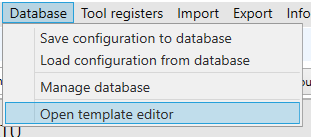
\includegraphics[width=0.4\textwidth]{../Img/Menu_Database.PNG}
    \caption{Menu Database}
\end{figure}

La finestra per inserire template personalizzati associati ai vari registri è la seguente:

\begin{figure}[H]
\centering
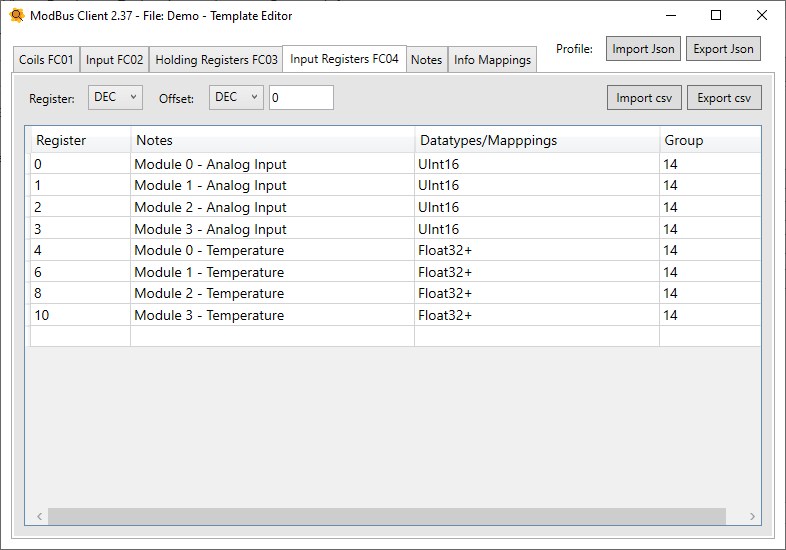
\includegraphics[width=0.80\textwidth]{../Img/ModBus_Client_Template_00.PNG}
\caption{Template editor}
\end{figure}

Per ogni registro nella finestra template si può associare un eventuale etichetta, 
il datatype corrispondente,
e se si desidera uno o più gruppi di risorse.
Nella stessa finestra è possibile specificare se i registri inseriti
sono da considerare in decimale o esadecimale ed un eventuale offset (positivo o negativo)
da aggiungere ai valori inseriti.
Ad esempio un offset di 100 sposta l'etichetta del registro 10 alla
posizione 110. Questo risulta comodo se, ad esempio, un PLC ha la \%MW0 che inizia all'offset
0x4000. In questo caso si compila la tabella partendo da 0 e poi è sufficiente impostare come
offset il valore HEX 4000. Nel caso in cui modelli diversi di PLC abbiano una posizione
diversa delle \%MW, per passare da un modello all'altro è
sufficiente cambiare l'offset senza dover andare a modificare i registri 
uno per uno
(si possono applicare anche offset negativi
qualora fosse necessario).
Si riportano a seguire gli screenshots di alcuni esempi basati sul template
dell'immagine precedente:

\begin{figure}[H]
\centering
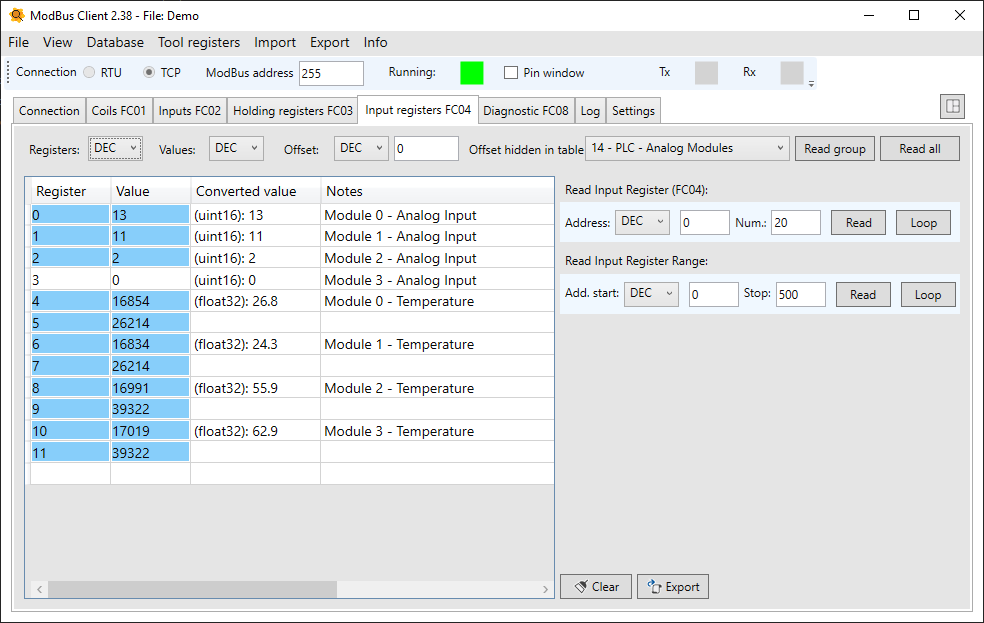
\includegraphics[width=0.70\textwidth]{../Img/ModBus_Client_Template_ReadDemo00.PNG}
\caption{Template editor}
\end{figure}

Nella colonna "Notes" vengono visualizzate le descrizioni dei vari registri 
mentre nella colonna "Converted Value" viene visualizzato il contenuto
di ciascun registro convertito nel datatype assegnatogli. In questo modo è molto semplice 
convertire valori a 32 o 64 bit, float o stringhe nel valore reale.
Selezionando un gruppo dal menu a tendina inoltre il client va a leggere i registri
del gruppo selezionato in ordine crescente.

Nella finestra template è possibile definire più gruppi di risorse e
associarli ai vari registri, in questo modo nella finestra principale si 
possono leggere registri diversi (anche non consecutivi)
richiamando il gruppo di risorse corrispondente.

\begin{figure}[H]
\centering
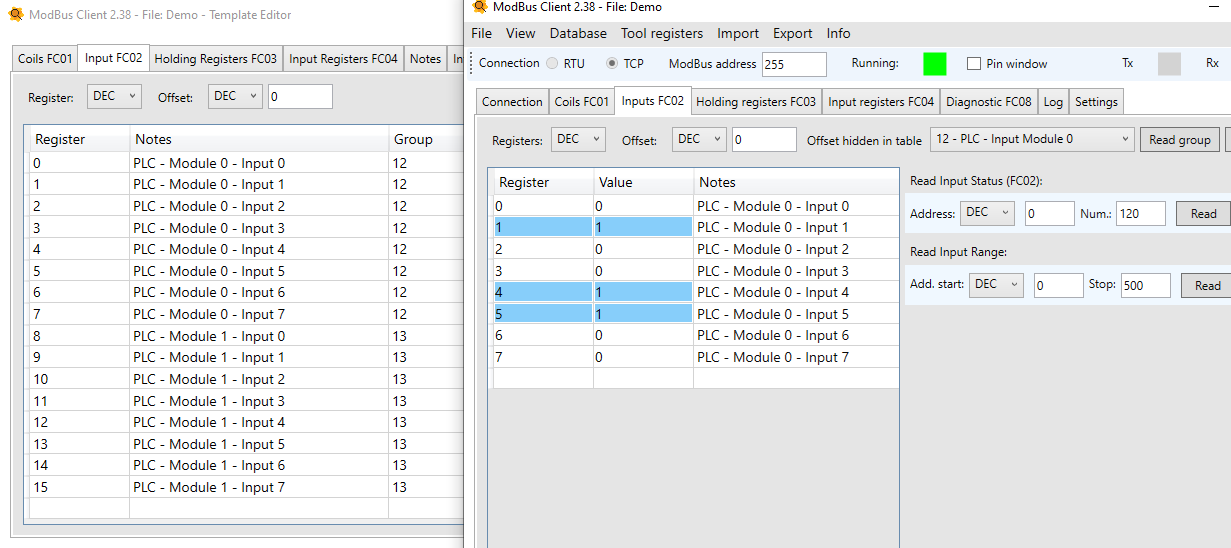
\includegraphics[width=0.85\textwidth]{../Img/ModBus_Client_Template_Group00.PNG}
\caption{Gruppi di risorse}
\end{figure}

\newpage
\section{Definizione gruppi}

Nella tab "Notes" della finestra template è possibile definire i gruppi di risorse
da richiamare poi nella finestra principale. Non è necessario inserire i gruppi in ordine.
La stessa tab mostra anche un riepilogo sul numero di registri e gruppi inseriti nel profilo.

\begin{figure}[H]
\centering
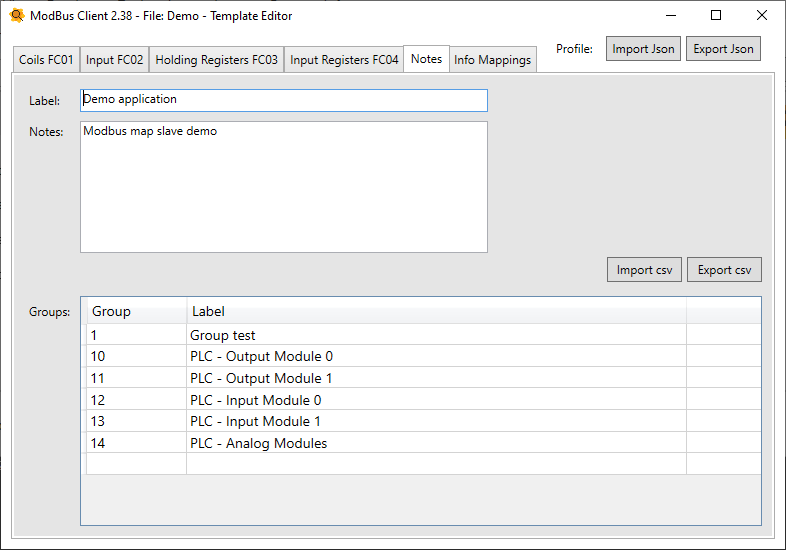
\includegraphics[width=0.70\textwidth]{../Img/ModBus_Client_Template_Group_Definition.PNG}
\caption{Definizione gruppi}
\end{figure}

L'ultima tab "Info Mappings" contiene un riepilogo dei datatypes implementati e gestiti dal client.

\begin{figure}[H]
\centering
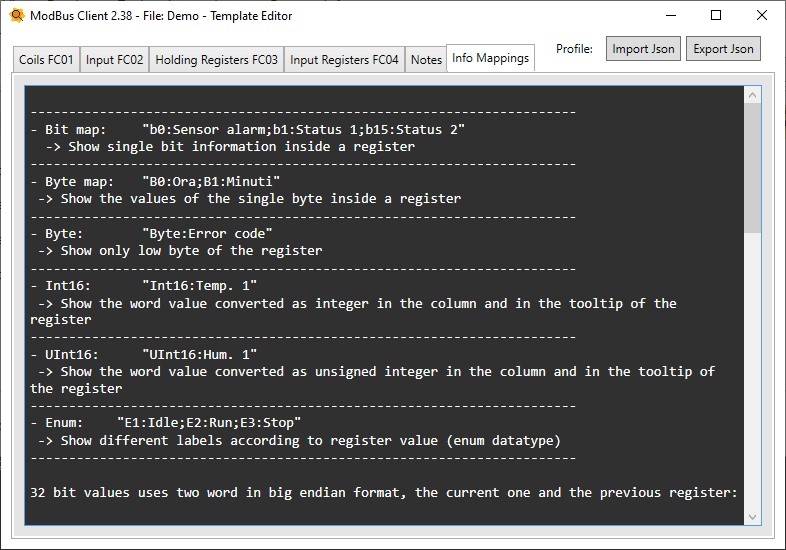
\includegraphics[width=0.70\textwidth]{../Img/ModBus_Client_Template_Info_Mappings.PNG}
\caption{Info Mappings}
\end{figure}

\newpage
\section{Datatypes}

Si riportano di seguito i vari datatypes supportati dal programma e configurabili nel template di un profilo.

\subsubsection{Bit map}

Mostra i singoli bit della word nella tooltip della riga con a fianco l'etichetta della risorsa.

\begin{verbatim}
    b0:Presenza tensione;b1:Stato 1;b15:Stato
\end{verbatim}

\subsubsection{Byte map}

Mostra i due byte della word nella tooltip della riga divisi per risorsa.

\begin{verbatim}
    B0:Ora;B1:Minuti
\end{verbatim}

\subsubsection{Int16 / UInt16}

Mostra la word con segno e visualizza il dato in int 16 nella tooltip della riga.

\begin{verbatim}
    Int16:Temp. 1
    UInt16:Counter
\end{verbatim}

Le variabili seguenti a 32 bit (due word) utilizzano la word del registro precedente (High Word) e
corrente (Low Word) a cui fa riferimento nel formato Big Endian.

\subsubsection{Float}

Raccoglie due word e visualizza il dato in float nella tooltip della riga.

\begin{verbatim}
    Float:Temperatura locale 1
\end{verbatim}

\subsubsection{Int32 / UInt32}

Raccoglie due word e visualizza il dato in int32 o uint32 nella tooltip della riga.

\begin{verbatim}
    Int32:Temperatura locale 1
    UInt32:Temperatura locale 2
\end{verbatim}

Le variabili seguenti a 64 bit (due word) utilizzano le tre word dei registri precedenti (High Word) e
corrente (Low Word) a cui fa riferimento nel formato Big Endian. Con i modificatori 
di formato è possibile specificare se utilizzare il registro corrente e i successivi tre.

\subsubsection{Int64 / UInt64}

\begin{verbatim}
    Int64:Timestamp start time
    UInt64:Timestamp start time
\end{verbatim}

\subsubsection{String(len[, offset])}

Con oggetti stringa è possibile convertire il contenuto dei registri
in stringa (NULL terminated string). Nell'esempio a seguire
vengono convertiti 8 byte in 8 caratteri ASCII con un offset di -2
(la stringa inizia dal registro precedente).

\begin{verbatim}
    String(8,-2):Modello
\end{verbatim}

\section{Modificatori del formato}

\subsubsection{Swap}

Aggiungendo un segno "-" o la stringa "\_swap" vengono utilizzate 
le due word invertite, in formato Little Endian.

\begin{verbatim}
    Swap: "UInt32-" "UInt32_swap"
\end{verbatim}

\subsubsection{Word offset}

Aggiungendo un segno "+" viene utilizzato il registro corrente come High Word e il successivo
come Low Word (Big Endian).

\begin{verbatim}
    Offset: "UInt32+"
\end{verbatim}

\subsubsection{Word offset + Swap}

\begin{verbatim}
    "UInt32-+" oppure "UInt32_swap+"
\end{verbatim}

Combina le due precedenti, usa il registro corrente e successivo nel formato Little Endian.

\newpage

Nell'esempio seguente si vedono 4 diversi mapping applicati al registro 102, come si vede nel caso
di conversioni di variabili a 32 bit si può scegliere quale word utilizzare per comporre il risultato
finale.
\\\\
Template:

\begin{figure}[H]
\centering
\includegraphics[width=0.75\textwidth]{../Img/Modbus_Client_Template_00.PNG}
\caption{}
\end{figure}

Esempio conversione finale:

\begin{figure}[H]
\centering
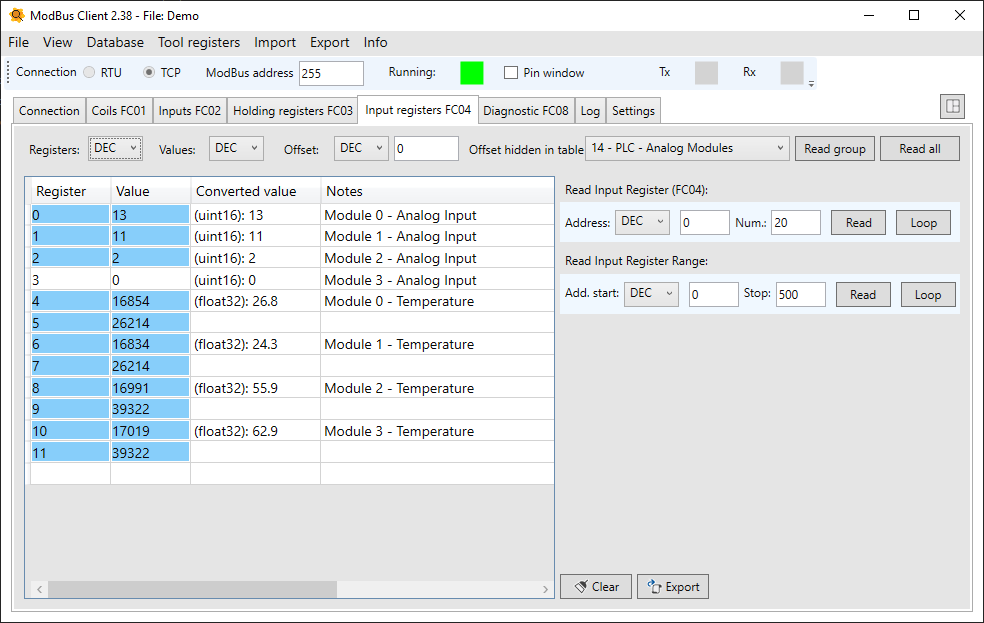
\includegraphics[width=0.75\textwidth]{../Img/ModBus_Client_Template_ReadDemo00.PNG}
\caption{}
\end{figure}
